%% LyX 2.3.0 created this file.  For more info, see http://www.lyx.org/.
%% Do not edit unless you really know what you are doing.
\documentclass[english]{article}
\usepackage[T1]{fontenc}
\usepackage[latin9]{inputenc}
\setlength{\parskip}{\smallskipamount}
\setlength{\parindent}{0pt}
\usepackage{float}
\usepackage{textcomp}
\usepackage{amsmath}
\usepackage{graphicx}
\usepackage{setspace}
\onehalfspacing

\makeatletter
%%%%%%%%%%%%%%%%%%%%%%%%%%%%%% Textclass specific LaTeX commands.
\newcommand{\lyxaddress}[1]{
	\par {\raggedright #1
	\vspace{1.4em}
	\noindent\par}
}

\makeatother

\usepackage{babel}
\begin{document}

\title{The Langmuir Model}

\author{Wei Tian}
\maketitle

\lyxaddress{TSMC}
\begin{abstract}
\noindent In this document, a feature scale model is developed and
used for recipe tuning. The detailed physical mechanisms and numerical
algorithms are introduced and discussed.\pagebreak{}
\end{abstract}
\tableofcontents{}\pagebreak{}

\section{Introduction - Langmuir Model}

Langmuir model is a comprehensive model simulating the plasma etching
processes. It consists of three sub-models, reactor model, sheath
model and feature model. Reactor model simulates the plasma in the
reactor scale, which is typically 30 to 50 cm. 

\section{File Structure}

Langmuir model is organized as a collection of three sub-models and
designed to use solvers as shared as possible. The file structure
is shown in the figure below, 

\begin{figure}[H]
\begin{centering}
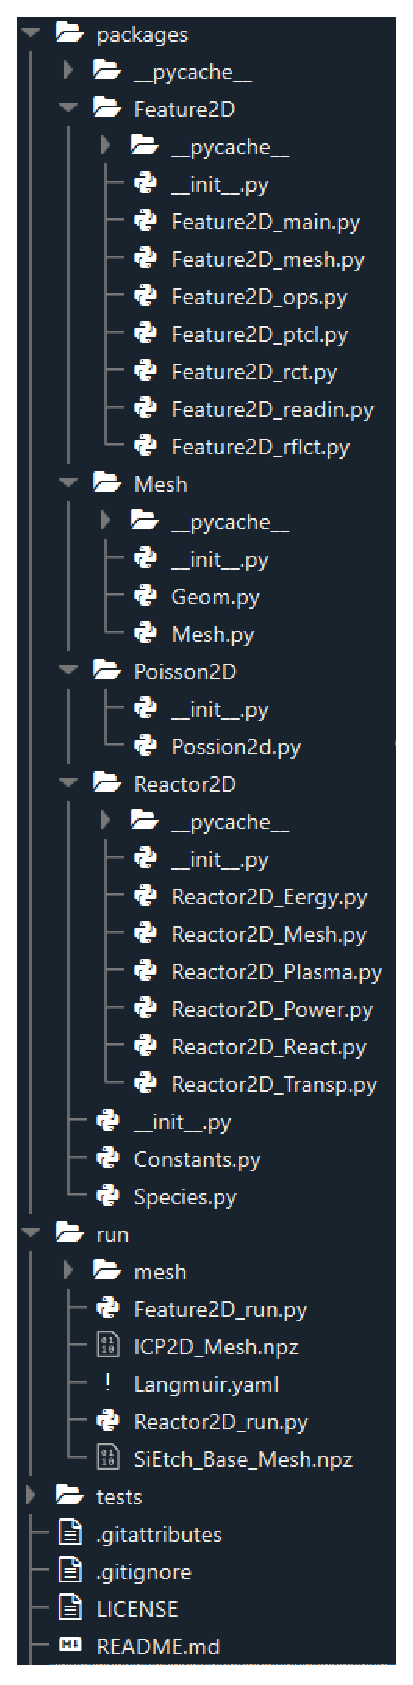
\includegraphics[scale=0.8]{Figures/Dir_Tree}
\par\end{centering}
\caption{The directory/file tree structure for Langmuir model. }
\end{figure}

Within the root directory, there are $packages$, where all the model
are placed, $run$, where applications/cases are run, and $tests$,
where model tests are tested and stored. License and Readme files
are placed in the root directory. Within the $packages$, $Reactor2D$,
$Sheath2D$ and $Feature2D$ directories contains model files for
each model, respectively. File naming follows the convention, $model\:name+2D+module\:name$.
$Constants.py$ and $Species.py$ are shared with all the three models,
so they are placed in the $packages$ level. As for its name, $Constants.py$
defines all constats, while $Species.py$ defines all species and
their properties. These are predefined varables, which are not supposed
to be changed or edited by users. $Mesh$ directory contains $Geom.py$
and $Mesh.py$ to create structured mesh, which in principle can be
used for any model requiring structured mesh, not limited to Langmuir
model. The $Mesh$ module can be either imported to each model or
used as a standalone one. When using as a standalone module, $Mesh$
saves all the information as $mesh.npz$ file. In reactor model, both
field module and transport module require a solver of Poisson-like
equation, therefore $Poisson2D$ is created at this level and works
as a general equation solver. The Poisson solver is also not limited
to Langmuir model. Within the $run$ directory, model run files are
placed. $Langmuir.yaml$ file serves as input file as all-in-one for
all three models. Within $tests$ directory, test are used by developers
and stored as benchmarks for the Langmuir model.

\section{Geometry and Mesh}

\subsection{Geometry}

\subsection{Mesh}

\section{Reactor Model}

\subsection{Introduction}

\subsection{Boltzmann Equation}

\subsection{Continuity Equation}

The fluid equation for plasma model is 
\[
\frac{\partial n}{\partial t}+\nabla\cdot\vec{\Gamma}=S
\]
\[
n-denisty
\]
\[
\vec{\Gamma}=n\vec{u}-flux
\]
\[
S-Source\:and\:loss\:term\:due\:to\:collisions
\]

The countinuity euqation is used for electron, ion and neutral spcies.
In order to solve for density $n$, two unknown terms are needed,
$\vec{\Gamma}$and $S$. Source term, $S$, is discussed in Sec. Chemistry.
Flux term, $\vec{\Gamma}$, can be solved by momentum equation,
\[
mn\frac{\text{\ensuremath{\partial}}}{\partial t}\vec{u}=eqn\vec{E}-\nabla p-mnv_{coll\_em}\vec{u}
\]
\[
\vec{u}-fluid\:velocity
\]
\[
m-mass
\]
\[
e-elementary\:charge
\]
\[
q-charge\:carried\:by\:species
\]
\[
\vec{E}-electric\:field
\]
\[
p-pressure
\]
\[
v_{coll\_em}-momentum\:collision\:frequency
\]

The magnetic field is ignored for most applications of low-temperature
plasmas and will addressed separately in another section. In the right-hand
side, the first term, $eqn\vec{E}$, represents the electric force.
The sencond term, $\nabla p$, represents. The thrid term, $mnv_{coll\_em}\vec{u}$,
is the momentum loss due to momentum collision. 

\subsubsection{Drift-Diffusion Appoximation}

The momentum equation is usually difficult to solve directly. A drift-diffusion
appoximation is widely used in plasma model. In we are only intersted
in steady-state plasmas, which results in $mn\frac{\text{\ensuremath{\partial}}}{\partial t}\vec{u}=0$,
the momentum equation can be writen as
\[
eqn\vec{E}-\nabla p-mnv_{coll\_em}\vec{u}=0
\]

where we assume that the background species is at rest and that the
momentum collision frequency, $v_{coll\_em}$, is a constant, independent
of velocity. Taking an isothermal plasma, such that $\nabla p=kT\nabla n$,
the momentume equation is writen as
\[
eqn\vec{E}-kT\nabla n-mnv_{coll\_em}\vec{u}=0
\]

now velocity, $\vec{u}$, is solvable,
\[
\vec{u}=\frac{eq\vec{E}}{mv_{coll\_em}}-\frac{kT}{mv_{coll\_em}}(\frac{\nabla n}{n})
\]
\[
\vec{\Gamma}=n\vec{u}=\frac{eqn\vec{E}}{mv_{coll\_em}}-\frac{kT\nabla n}{mv_{coll\_em}}
\]
\[
\vec{\Gamma}=\frac{q}{|q|}\mu n\vec{E}-D\nabla n
\]
\[
\mu=\frac{e|q|}{mv_{coll\_em}}\;-\;mobility
\]
\[
D=\frac{kT}{mv_{coll\_em}}\;-\;diffusivity,\:diffusion\:coefficient
\]

The first term, $e\mu n\vec{E}$, represents the drift term; the sencond
term, $D\nabla n$, represents the diffusion term. That is where the
name of appoximation comes from.

E-field in the continuity equation is derived by potential, $\vec{E}=-\nabla\phi$,
continuity equation can be written in terms of density and potential,
\[
\frac{\partial n_{e}}{\partial t}=-\mu_{e}n\vec{_{e}E}-D_{e}\nabla n_{e}+S_{e}=f_{e}(n_{e}(t),\phi(t))
\]
\[
\frac{\partial n_{i}}{\partial t}=q_{i}\mu_{i}n\vec{_{i}E}-D_{i}\nabla n_{i}+S_{i}=f_{i}(n_{i}(t),\phi(t))
\]
\[
-\nabla\cdot\varepsilon\nabla\phi(t)=e(\sum_{i}n_{i}(t)-n_{e}(t))
\]

In this form, the future density $n_{e}(t1)$ is determined by current
density, $n_{e}(t0)$ , and current potential, $\phi(t0)$. The current
potential, $\phi(t0)$, is determined by the toall charge density,
$\sum_{i}n_{i}(t)-n_{e}(t)$. Explicitly, the equations above can
be solved through iterative method. Given initial densities, $n_{e}(t0)$
and $n_{i}(t0)$, initial potnetial $\phi(t0)$can be solved. By putting
densities and potential into continuity equation, the densities $n_{e,i}(t1)$
at next time, $t1$, can be obtained. The more detailed discussion
can be found in the sec. Poisson's Equation.

\subsubsection{Ambipolar Appoximation}

In the steady state where the background gas is dominant, we make
the congruence assumption that the flux of electrons and ions out
of any region must be equal, $\vec{\Gamma}_{e}=\vec{\Gamma}_{i}$,
such that charge does not build up. This is still true in the presence
of ionizing collisions, which create equal numbers of both negative
and positive species. Since the electrons are ligher, and would tend
to flow out faster (in an unmagnetized plasma), an electric field
must spring up to maintain the local flux balance. That is, a few
more electrons than ions initially leave the plasma region to set
up a charge imbalance and consequently an electric field. Let's expand
the flux balance, $\vec{\Gamma}_{e}=\vec{\Gamma}_{i}$,
\[
-\mu_{e}n_{e}\vec{E}-D_{e}\nabla n_{e}=\mu_{i}n_{i}\vec{E}-D_{i}\nabla n_{i}
\]
Note that the drift term is negative for electrons and positive for
ions, where E-field drags electrons down and speed ions up to balance
the fluxes. Assume charge neutrality in space, $n_{e}=n_{i}$, E-field
can be solved as
\[
\vec{E}_{ambi}=\vec{E}=\frac{D_{i}-D_{e}}{\mu_{i}+\mu_{e}}(\frac{\nabla n_{e}}{n_{e}})
\]

This E-field is called ambipolar E-field and substituted to the flux,
\[
\vec{\Gamma}_{e,i}=\mu_{i}\frac{D_{i}-D_{e}}{\mu_{i}-\mu_{e}}\nabla n_{e}-D_{i}\nabla n_{e}=-\frac{\mu_{e}D_{i}+\mu_{i}D_{e}}{\mu_{i}+\mu_{e}}\nabla n_{e}
\]

You can see the coefficient is symmetric, and equal to electron and
ion. A new diffusion coefficient can be defined as
\[
D_{ambi}=\frac{\mu_{e}D_{i}+\mu_{i}D_{e}}{\mu_{i}+\mu_{e}}
\]
\[
\vec{\Gamma}_{e,i}=-D_{ambi}\nabla n_{e}
\]
\[
\mu_{e}=\frac{|q|}{v_{coll\_em}}(\frac{1}{m_{e}})\gg\mu_{i}=\frac{|q|}{v_{coll\_em}}(\frac{1}{m_{i}}),\:since\:m_{e}\ll m_{i}
\]
\[
D_{ambi}\approx D_{i}+\frac{\mu_{i}}{\mu_{e}}D_{e}=D_{i}(1+\frac{T_{e}}{T_{i}})
\]

put it back to the continuity equation,
\[
\frac{\partial n}{\partial t}+D_{ambi}\nabla^{2}n=S
\]

Now the continuity becomes a standard DIFFUSION equation with source
term, and much easier to solve. When using ambipolar diffusion appoximation,
we only calculate ion density $n_{i}$, and enforce charge neutrality,
$n_{e}=n_{i}$. Ambipolar E-field, $E_{ambi}$, can be used for electron
energy equation. In this way, Poisson's equation is avoided.

\subsection{Poisson's Equation}

\subsubsection{Explicit Poisson's equation}

With explict method, the potenital in the Poisson's equation is determined
by the current charge density, which is impacted by the prevous potential.
\[
-\nabla\cdot\varepsilon\nabla\phi(t)=e(\sum_{ion}n_{i}(t)-n_{e}(t))
\]
\[
-\nabla\cdot\varepsilon\nabla\phi(t+\Delta t)=e(\sum_{ion}n_{i}(t+\Delta t)-n_{e}(t+\Delta t))
\]
\[
\dfrac{\partial n_{e,i}}{\partial t}=D_{e,i}\nabla^{2}n_{e,i}(t)\pm\nabla\cdot(\mu_{e,i}n_{e,i}(t)\nabla\phi(t))+S_{e}(t)
\]

\[
n_{e,i}(t+\Delta t)=n_{e,i}(t)+\Delta t\times f_{e,i}(\phi(t))
\]
\[
-\nabla\cdot\varepsilon\nabla\phi(t+\Delta t)=F(\phi(t))
\]

where
\[
\phi=potenital
\]
\[
\varepsilon=permittivity
\]
\[
e=elementary\:charge
\]

\[
n_{e,i}=electron,ion\:density
\]
\[
\mu_{e,i}=electron,ion\:mobility
\]

with the derivation above, the future potential is determined by the
current potenital.

\subsubsection{Semi-implicit electron with predictor-corrector ions}

The timestep is limited to as small as a few picoseconds, which is
not practical for any useful simulations. Implicit method can theoretically
remove the limit of the timestep, with the cost of solving for the
reversed matrix. The matrix solver could be much expensive as well.
A semi-implict method is, therefore, proposed to increase the timestep
and meanwhile reduce the cost of matrix solver. The principal is shown
as below, 
\[
-\nabla\cdot\varepsilon\nabla\phi(t+\Delta t)=e(\sum_{ion}n_{i}(t+\Delta t)-n_{e}(t+\Delta t))
\]
\[
\dfrac{\partial n_{e}}{\partial t}=D_{e}\nabla^{2}n_{e}(t)-\nabla\cdot(\mu_{e}n_{e}(t)\nabla\phi(t+\Delta t))+S_{e}(t)
\]
\[
n_{e}(t+\Delta t)=n_{e}(t)+\Delta t\times f_{e}(\phi(t+\Delta t))
\]
\[
\dfrac{\partial n_{i}}{\partial t}=D_{i}\nabla^{2}n_{i}(t)+\nabla\cdot(\mu_{i}n_{i}(t)\nabla\phi(t))
\]
\[
n_{i}(t+\Delta t)=n_{i}(t)+\Delta t\times f_{i}(\phi(t))
\]
\[
-\nabla\cdot\varepsilon\nabla\phi(t+\Delta t)=e(\sum_{ion}[n_{i}(t)+f_{i}(\phi(t))]-[n_{e}(t)+f_{e}(\phi(t+\Delta t))])
\]
\[
-\nabla\cdot\varepsilon\nabla\phi(t+\Delta t)=
\]
\[
e(\sum_{ion}[\underline{n_{i}(t)+\Delta t\times f_{i}(\phi(t))}]-\Big[\underline{n_{e}(t)+\Delta t\times S_{e}(t)+\Delta t\times D_{e}\nabla^{2}n_{e}(t)-\Delta t\times\nabla\cdot(\mu_{e}n_{e}(t)\nabla\phi(t+\Delta t))}\Big])
\]
\[
-\nabla\cdot\varepsilon\nabla\phi(t+\Delta t)+e\times\Delta t\times\nabla\cdot(\mu_{e}n_{e}(t)\nabla\phi(t+\Delta t))=F(n_{e,i}(t),\phi(t))
\]
\[
\Big[\underline{-\nabla\varepsilon\cdot\nabla\phi(t+\Delta t)-\varepsilon\nabla^{2}\phi(t+\Delta t)}\Big]+\Big[\underline{(e\mu_{e}\Delta t)\nabla n_{e}(t)\cdot\nabla\phi(t+\Delta t)+(e\mu_{e}\Delta t)n_{e}(t)\nabla^{2}\phi(t+\Delta t)}\Big]
\]
\[
=F(n_{e,i}(t),\phi(t))
\]
\[
[\underline{(e\mu_{e}\Delta t)n_{e}(t)-\varepsilon}]\nabla^{2}\phi(t+\Delta t)+[\underline{(e\mu_{e}\Delta t)\nabla n_{e}(t)-\nabla\varepsilon}]\cdot\nabla\phi(t+\Delta t)=F(n_{e,i}(t),\phi(t))
\]
\[
\underline{A(n_{e}(t))}\nabla^{2}\phi(t+\Delta t)+\underline{\nabla B(n_{e}(t))}\cdot\nabla\phi(t+\Delta t)=F(n_{e,i}(t),\phi(t))
\]
\[
underline-emphasis
\]

The electron density is solved using implicit method, where the future
electron density is determined by the future potential, while the
ion density is still solved using explicit method, where the future
ion density is determined by the current potential. In this scenario,
electron denisty and potential get quickly convergent with large timestep.
A further attension needs to be payed to the ion density, which could
oscillate. The predictor-corrector method is used for ion density.
\[
\tilde{n}_{i}(t+\Delta t)=n_{i}(t)+\Delta t\times f_{i}(n_{i}(t),\phi(t))
\]
\[
n_{i}(t+\Delta t)=n_{i}(t)+\Delta t\times\dfrac{1}{2}(f_{i}(n_{i}(t),\phi(t))+f_{i}(\tilde{n}_{i}(t+\Delta t),\phi(t+\Delta t)))
\]


\subsubsection{Semi-implicit Poisson's equation}

The ion density can use implicit method as well. In this case, 
\[
-\nabla\cdot\varepsilon\nabla\phi(t+\Delta t)=e(\sum_{ion}[\underline{n_{i}(t)+f_{i}(\phi(t+\Delta t))}]-[\underline{n_{e}(t)+f_{e}(\phi(t+\Delta t))}])
\]
\[
-\nabla\cdot\varepsilon\nabla\phi(t+\Delta t)=e(\sum_{e,i}[\underline{n_{e,i}(t)+f_{e,i}(\phi(t+\Delta t))}]
\]
\[
-\nabla\cdot\varepsilon\nabla\phi(t+\Delta t)=
\]
\[
e(\sum_{e,i}\Big[\underline{n_{e,i}(t)+\Delta t\times S_{e,i}(t)+\Delta t\times D_{e,i}\nabla^{2}n_{e,i}(t)+\Delta t\times\nabla\cdot(q\mu_{e,i}n_{e,i}(t)\nabla\phi(t+\Delta t))}\Big])
\]
\[
-\nabla\cdot\varepsilon\nabla\phi(t+\Delta t)-\sum_{e,i}\Delta t\times\nabla\cdot(eq\mu_{e,i}n_{e,i}(t)\nabla\phi(t+\Delta t))=F(n_{e,i}(t))
\]
\[
[\underline{\sum_{e,i}(eq\mu_{e,i}\Delta t)n_{e,i}(t)-\varepsilon}]\nabla^{2}\phi(t+\Delta t)+[\underline{(e\Delta t)\sum_{e,i}\mu_{e,i}\nabla n_{e,i}(t)-\nabla\varepsilon}]\cdot\nabla\phi(t+\Delta t)=F(n_{e,i}(t))
\]
\[
\underline{A(n_{e,i}(t))}\nabla^{2}\phi(t+\Delta t)+\underline{\nabla B(n_{e,i}(t))}\cdot\nabla\phi(t+\Delta t)=F(n_{e,i}(t))
\]

The future potential is solved directly, which means that the future
potential does not depends on the current potential anymore. All coefficients
in this equation are densities at current time. The second term in
the LHS is probably (not sure, need addtional check) not easy to deal
with. It could be rewritten in explicit form and moved to the RHS.
\[
\underline{A(n_{e,i}(t))}\nabla^{2}\phi(t+\Delta t)+\underline{\nabla B(n_{e,i}(t))}\cdot\nabla\phi(t+\Delta t)=F(n_{e,i}(t))
\]
\[
\underline{A(n_{e,i}(t))}\nabla^{2}\phi(t+\Delta t)=F(n_{e,i}(t))+\underline{\nabla B(n_{e,i}(t))}\cdot\nabla\phi(t)
\]
\[
\underline{A(n_{e,i}(t))}\nabla^{2}\phi(t+\Delta t)=F(n_{e,i}(t),\phi(t))
\]

Now the Poisson's equation retains its Lapalacian form, with the source
term depending on current potential. The same technique can be applied
to Sec. 3.2 as well.

\subsection{Momentum Equation}

\subsubsection{Plasma Conductivity}

Consider a small-amplitude perturbation of electromagnetic field,
having an electric field in the x-direction of an infinite plasma.
The electric field may be defined using complex numbers: $E=E_{0}cos(i\omega t)$.
In a typical plasma etching application, $\omega=2\pi f$, where $f=13.56$
MHz. Let's look at the electron momentum equation,
\[
m_{e}n_{e}\frac{\text{\ensuremath{\partial}}}{\partial t}u_{e}=-en_{e}E_{0}cos(i\omega t)-\nabla p_{e}-m_{e}n_{e}v_{coll\_em}u_{e}
\]

With the assumption that :
\begin{enumerate}
\item the ions do not respond to this high-frequency perturbation
\item the electron pressure gradient is not significant, effectively ignoring
electron thermal energy 
\item there is no steady current in the plasma so the drift speed is zero 
\item electron velocity follows the same oscillation, $u=u_{0}cos(i\omega t)$.
\end{enumerate}
The electron momentum equation linearizes to
\[
(n_{e}m_{e}i\omega)u_{0}cos(i\omega t)=\text{\textminus}n_{e}eE_{0}cos(i\omega t)\text{\textminus}(n_{e}m_{e}v_{coll\_em})u_{0}cos(i\omega t)
\]

The magnitudes of the perturbations in velocity and electric field
amplitude are therefore related by 
\[
u_{0}=\text{\textminus}\frac{e}{m_{e}(i\omega+v_{coll\_em})}E_{0}
\]

current is determined by
\[
J_{0}=\text{\textminus}en_{e}u_{0}=\frac{e^{2}n_{e}}{m_{e}(i\omega+v_{coll\_em})}E_{0}
\]

The electron conductivity $\sigma_{e}$ is, 
\[
\sigma_{e}=\frac{e^{2}n_{e}}{m_{e}(i\omega+v_{coll\_em})}
\]

Plasma conductivity $\sigma_{plasma}=\sigma_{e}+\sigma_{ion}\approx\sigma_{e}$,
since $\sigma_{e}\gg\sigma_{ion}$.

Notice that when collision dominates the plasma, $v_{coll\_em}\gg\omega$,
$\sigma_{e}=\frac{e^{2}n_{e}}{m_{e}v_{coll\_em}}$, $\sigma_{e}$
is real. Current is synchronized in phase with E-field and power is
absoped by the electron. When oscillation dominates the plasma, $\omega\gg v_{coll\_em}$,
$\sigma_{e}=-i\frac{e^{2}n_{e}}{m_{e}\omega}$, $\sigma_{e}$ is imaginary.
Current is $90^{\circ}$ lagged in phase with E-field so that power
is reflected by the electron.

\subsection{Electon Energy Equation}

The energy conservation equation is obtained by multiplying the Boltzmann
equation by kinectiv energy, $\frac{1}{2}mv^{2}$, and integrating
over velocity,
\[
\frac{\partial}{\partial t}(\frac{3}{2}n_{e}kT_{e})+\nabla\cdot Q_{e}=P_{in}-P_{loss}
\]
\[
\frac{3}{2}n_{e}kT_{e}-thermal\:energy\:density\:(J/m^{3})
\]
\[
k-Boltzmann\:Constant
\]
\[
Q_{e}-energy\:flux\:(W/m^{2}),\:Q_{e}=\frac{5}{2}kT_{e}\Gamma_{e}-k_{e}\nabla T_{e}
\]
\[
k_{e}-thermal\:conductivity,\:k_{e}=3kD_{e}n_{e}/2
\]
\[
D_{e}-electron\:diffusion\:coefficient
\]
\[
P_{in}-Power\:Input,\:P_{loss}-Power\:Loss
\]

The form of energy equation, where energy density is solved, is similar
to that of continuity equation, where species density is solved. Energy
flux, $Q_{e},$consists of two terms, in which $\frac{5}{2}kT_{e}\Gamma_{e}$
represents the themal convection and $k_{e}\nabla T_{e}$ represents
the themeral conduction. The input power includes both external and
internal energy flowing into the electrons. The source can come from
electric field, electron beam, or photons. Under the assumption of
resistive plasma where Ohm heating (also called Joule heating/resistive
heating) dominates, 
\[
P_{in}=\sigma E^{2}
\]
\[
\sigma-Plasma\:Conductivity,\:(S/m)
\]
\[
E-Electric\:Field,\:including\:both\:external\:and\:internal\:field
\]

External electric field is obtained from the the Field Solver and
interal electric field is obtained from the Transport Solver. In plasma,
power gets lost mainly through energy flow to the walls and electron-impact
collisions. The former loss is included in the $\nabla\cdot Q_{e}$
term. The collision loss can be seen as below, 
\[
P_{loss}=3\frac{m_{e}}{M}n_{e}kv_{coll\_em}(T_{e}-T_{g)+n_{e}N\sum_{j}k_{j}(T_{e})\Delta\varepsilon_{j}}
\]
The first term, $3\frac{m_{e}}{M}n_{e}kv_{coll\_em}(T_{e}-T_{g})$,
is due to electron elastic collision (also called momentum collision),
in which no reaction occurs. For elastic collsion, the electron energy
loss can be derived from momentum and energy conservation equations
for 2-body collision. The second term, $n_{e}N\sum_{j}k_{j}(T_{e})\Delta\varepsilon_{j}$,
counts for the inelastic collisions, in which reactions, such as excitation
and ionization, occur. 

The boundary conditions of the electron energy towards the wall were
taken as
\[
Q_{e}(at\:b.c.)=\frac{5}{2}kT_{e}\Gamma_{e}(at\:b.c.)\cdot\hat{n}
\]
\[
\text{\ensuremath{\hat{n}-surface\:normal\:vector}}
\]

At the wall surface, energy which is normal with respect to the surface
is lost completely.

\subsection{Electron Energy Distribution Function}

\subsubsection{Null-collision technique}

The electron energy and collision frequency can change during the
free flight between collisions. There is an ambiguity in choosing
the time between collisions, seen in the figure below. 
\begin{figure}[H]
\begin{centering}
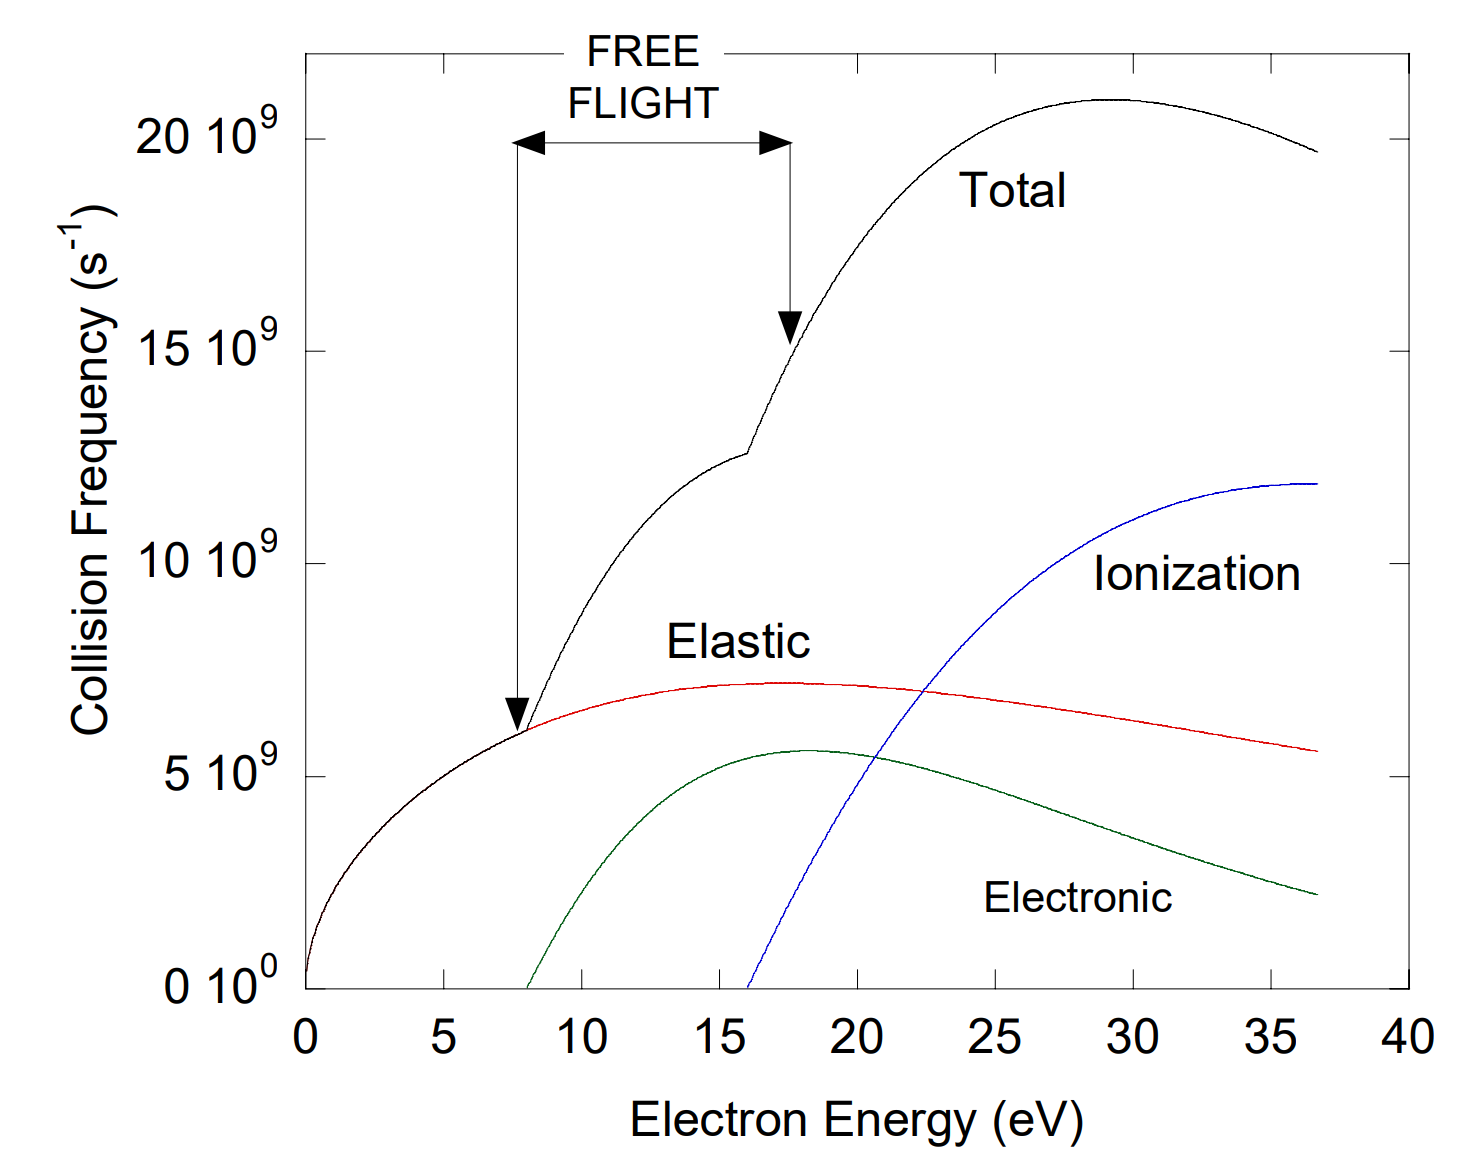
\includegraphics[scale=0.2]{Figures/Null-Collision}
\par\end{centering}
\caption{Free flight time changes during the flight.}

\end{figure}

The ambiguity is eliminated by the \textquotedblleft null collision
frequency\textquotedblright{} (NCF). The null-collision concept is
introduced into the direct-simulation Monte Carlo method in the rarefied
gas dynamics. The null-collision technique overcomes the principle
fault in the time-counter technique and the difficulties in the collision-frequency
technique. The computation time required for the null-collision technique
is comparable to that for the time-counter technique. Therefore, it
is concluded that the null-collision technique is superior to any
other existing techniques in the direct-simulation Monte Carlo method.

The NCF is a fictitious process used to make it appear that all energies
have the same collision frequency.
\[
v_{null}(\varepsilon)=max_{\varepsilon}[v_{total(\varepsilon)}]-v_{total}(\varepsilon)
\]
\[
xs_{null}(\varepsilon)=max_{\varepsilon}[xs_{total}(\varepsilon)]-xs_{total}(\varepsilon)
\]
\[
v-collision\:frequency
\]
\[
xs-cross\:section
\]

When collision falls to the ``Null Collision'', there is no impact
on the electron, which proceeds to the next free flight time without
changing its velocity. The ``Null Collision'' frequency and cross
section can be seen as below,
\begin{figure}[H]
\begin{centering}
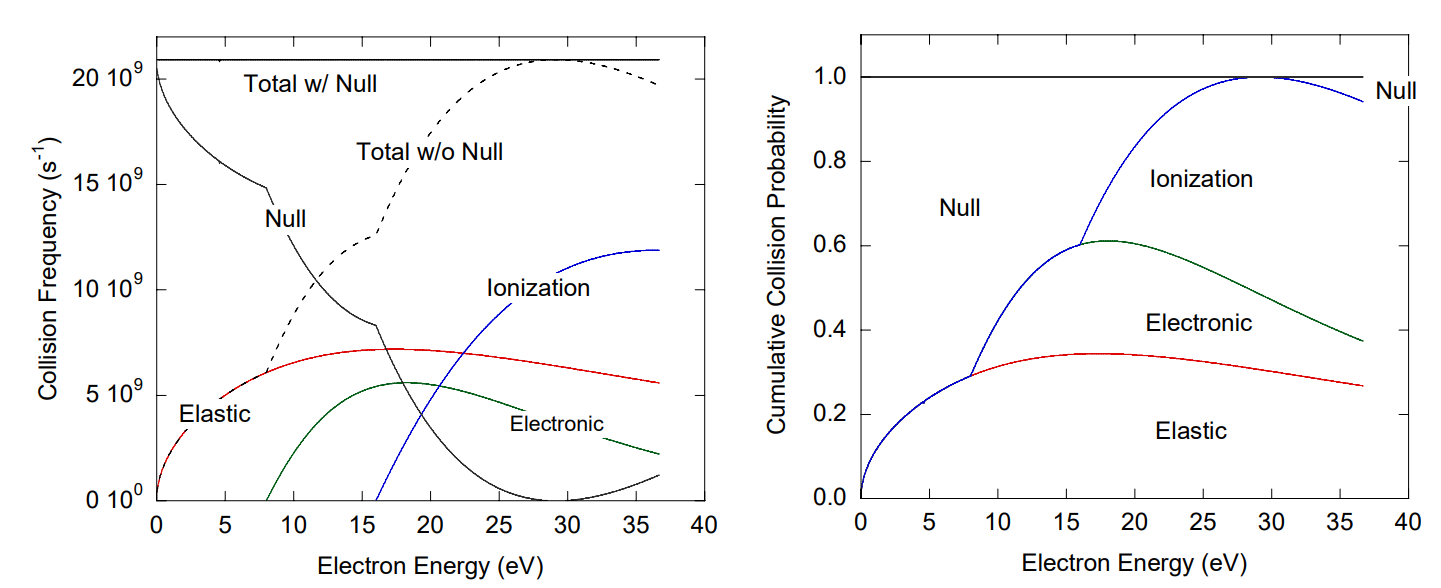
\includegraphics[scale=0.3]{Figures/Null-Collision-frequency}
\par\end{centering}
\caption{The collision frequency and cross section of ``Null Collision''.}

\end{figure}

The free flight time between collisions is determined by the maximum
total collision frequency. 
\[
\Delta t=\frac{-1}{max_{\varepsilon}[v_{total}(\varepsilon)]}log(1-r_{1})
\]

The collision which occurs is that which satisfies
\[
p_{j-1}(\varepsilon)<r_{2}\le p_{j}(\varepsilon)
\]
\[
p_{j}-the\:pth\:collision\:process
\]

\begin{figure}[H]
\begin{centering}
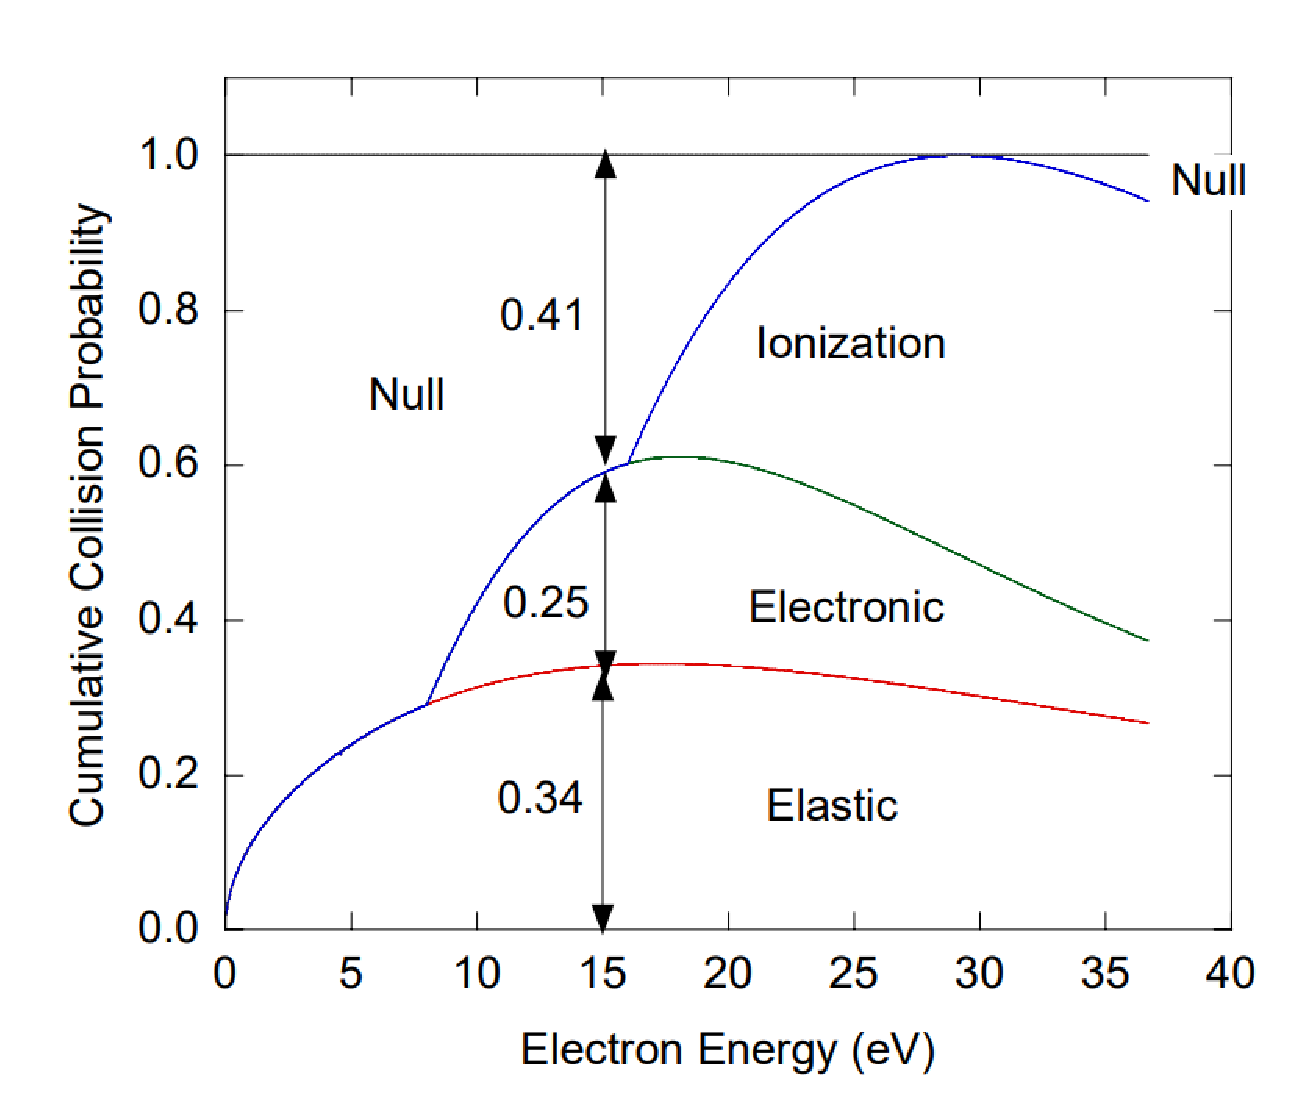
\includegraphics[scale=0.5]{Figures/Null-Collision-choose}
\par\end{centering}
\caption{Collision process chosen according to the cumulative probability.}

\end{figure}


\subsection{Chemistry}

\subsubsection{Introduction}

In the continuity equation, there is a source term in the right hand
side,
\[
\frac{\partial n}{\partial t}+\nabla\cdot\Gamma=S
\]
\[
n-density\:of\:any\:species,\:such\:as\:electron,\:ion\:and\:neutrals
\]
\[
\Gamma-flux\:of\:any\:species,\:such\:as\:electron,\:ion\:and\:neutrals
\]
\[
S-source\:term\:of\:species\:due\:to\:reactions
\]

The flux term has been discussed in the previous section. The source
term, $S$, here refers to the volume production and sink of a given
species. The source term due to surface reaction will be discussed
later. 

Usually, reactions can be written as following form,
\[
A+B+C+...\rightarrow a+b+c+...
\]
\[
left-reactants,\:right-products
\]

For any species appeared in the left hand side, the reaction serves
as a sink for that species; for any species appeared in the right
hand side, the reaction serves as a production for that species. The
reaction rate can be calculated as,
\[
R=k\times n_{A}\times n_{B}\times n_{C}\times...
\]
\[
R-reaction\:rate
\]
\[
k-reaction\:rate\:coefficient
\]
\[
n_{A}-density\:of\:species\:A
\]

Let us take an example. In Ar discharge, a basic reactions set includes
electron-impact excitation, ionization and Penning ionization,
\[
Electron-Impact\:Ionization:\;e+Ar\rightarrow Ar^{+}+e+e
\]
\[
Electron-Impact\:Excitation:\;e+Ar\rightarrow Ar^{*}+e
\]
\[
Penning\:Ionization:\;Ar^{*}+Ar^{*}\rightarrow Ar+Ar^{+}+e
\]
\[
Ar^{*}-excited\:Ar\:state
\]

For electron, the source term will include first and third reactions.
The second reaction loses an electron in the left side and produce
one in the right side, resulting net gain or loss. In the electron-impact
ionization, one electron is consumed while two electrons are produced,
resulting in net gain of one electron. Penning ionization produces
one electron. The source term for electron is 
\[
S_{e}=k_{ioniz}\times n_{e}\times n_{Ar}+k_{pen}\times n_{Ar^{*}}^{2}
\]

Similarly, the source terms for ion, $S_{Ar^{+}}$, and for excited
state, $S_{Ar^{*}}$, can be calculated as
\[
S_{Ar^{+}}=k_{ioniz}\times n_{e}\times n_{Ar}+k_{pen}\times n_{Ar^{*}}^{2}
\]
\[
S_{Ar^{*}}=k_{exc}\times n_{e}\times n_{Ar}-2\times k_{pen}\times n_{Ar^{*}}^{2}
\]

In this simple reaction set, electron-ion pair is always created simultaneously
so that $S_{Ar^{+}}=S_{e}$ everywhere. 

When the source term is added to plasma transport equation, it could
result in different coupling depending on the way to process it. For
example, using the Ar discharge defined above, 
\[
\frac{\partial n_{e}}{\partial t}+\nabla\cdot\Gamma_{e}(n_{e})=S_{e}
\]
\[
\frac{\partial n_{e}}{\partial t}+\nabla\cdot\Gamma_{e}(n_{e})=k_{ioniz}n_{e}n_{Ar}+k_{pen}n_{Ar^{*}}^{2}
\]

In the first equation, $S_{e}$can be used as a constant source which
is computed from a fixed electron density. In the second equation,
$S_{e}$is treated as a function of $n_{e}$, which means that $n_{e}$
is needed to be solved at the same time as left-hand side. Since the
source term, $S_{e}$, is a linear function of $n_{e},$the complexity
does not increase much. However, when it comes to the transport equation
for ions, coupling effect has to be counted. 
\[
\frac{\partial n_{i}}{\partial t}+\nabla\cdot\Gamma_{i}(n_{i})=k_{ioniz}n_{e}n_{Ar}+k_{pen}n_{Ar^{*}}^{2}
\]

The left-hand side is a function of $n_{i}$ while the right-hand
side if a function of $n_{e}$. It means that $n_{e}$ and $n_{i}$
need to be solved simultaneously. Furthermore, all species, $n_{e}$,
$n_{i}$and $n_{Ar^{*}}$ need to be solved at the same time. 
\[
\frac{\partial n_{e}}{\partial t}+\nabla\cdot\Gamma_{e}(n_{e})=k_{ioniz}n_{e}n_{Ar}+k_{pen}n_{Ar^{*}}^{2}
\]
\[
\frac{\partial n_{i}}{\partial t}+\nabla\cdot\Gamma_{i}(n_{i})=k_{ioniz}n_{e}n_{Ar}+k_{pen}n_{Ar^{*}}^{2}
\]
\[
\frac{\partial n_{Ar^{*}}}{\partial t}+\nabla\cdot\Gamma_{Ar^{*}}(n_{Ar^{*}})=k_{exc}n_{e}n_{Ar}-2k_{pen}n_{Ar^{*}}^{2}
\]

The three equations are coupled together and all densities need to
be solved simultaneously. 

\subsubsection{Electron Impact Reaction}

Assuming electron follows the Maxwellian distribution, reaction rate
coefficients are modeled using Arrenhius form, which is 
\[
k_{e}(T_{e})=A\times T_{e}^{n}\times exp(-\frac{E_{act}}{T_{e}})
\]
\[
k_{e}-rate\:coefficient
\]
\[
A-Arrenhius\:coefficient,1st\:order:\:in\:1/s;\:2nd\:order:\:in\:m^{3}/s
\]
\[
T_{e}-electron\:temperature,\:in\:eV
\]
\[
E_{act}-activation\:energy,\:in\:eV
\]

When electron energy distribution cannot be assumed Maxwellian distribution,
reaction rate coefficients have to be computed by electron energy
module.

\subsubsection{Heavy Particle Reaction}

For heavy particle reactions with no electron in reactants, the Arrenhius
form can also be used for rate coefficients. 

\[
Rate\:coeff=A\times(\frac{T}{298})^{n}\times exp(-\frac{E_{ref}}{T})
\]
\[
A-Arrenhius\:coefficient,1st\:order:\:in\:1/s;\:2nd\:order:\:in\:m^{3}/s
\]
\[
T-gas\:temperature,\:in\:K
\]
\[
E_{ref}-reference\:energy,\:in\:K
\]


\section{Sheath Model}

\subsection{Introduction}

When plasmas with quasi-neutrality ($n_{e}\approx n_{i}$) are joined
to wall surfaces, a positively charged layer called $sheath$ is required
in physics to maintain the balance of electrons and ions. The electron
thermal velcocity $(eT_{e}/m_{e})^{1/2}$ is at least 100 times the
ion thermal velocity $(eT_{i}/m_{i})^{1/2}$, as $T_{e}\ge T_{i}$
and $m_{e}\ll m_{i}$ . Let us assume an initial plasma with zero
electric potenital and E-field everywhere, since $n_{e}=n_{i}$at
$t=0$. The electrons are not confined by any field or potential and
hence move faster to the walls than ions. On a short timescale, some
electrons near the walls are lost, leading to net positive space charges
near the walls. This positively charged space, which is SHEATH, creates
an E-field pointing to the walls, reducing the electron speed and
increasing the ion speed to the walls. Eventually, the loss of electrons
and ions balance each other and plasma remains quasi-neutral. Sheath
plays an important role in the plasma etching. As positive ions flowing
out of the bulk plasma enter the sheath, they get accelerated by the
sheath fields and pick up high energies as they traverse across the
sheath. The ions carry these high energies and delivers to the materials
surface, such as Si surface. The ion etch rates, selectivity and damage
are also impacted by the energies, which are determiend by the sheath.
A diagram of sheath can be seen in the figure below.

Within the Langmuir model, Sheath model serves as a connector between
Reactor model and Feature model. It takes the E-filed and species
from the Reactor model and compute the angular and energy distribution
of electrons and ions, which is fed into the Feature model as input.
Sheath model uses particle tracing algorithm and basically traces
particles under varying E-field. Particle collisions are taken into
account and they widen the distribution of angle. In the code structure,
modules from Feature model, such as particle and move, can be shared
with Sheath model.

\begin{figure}[H]
\begin{centering}
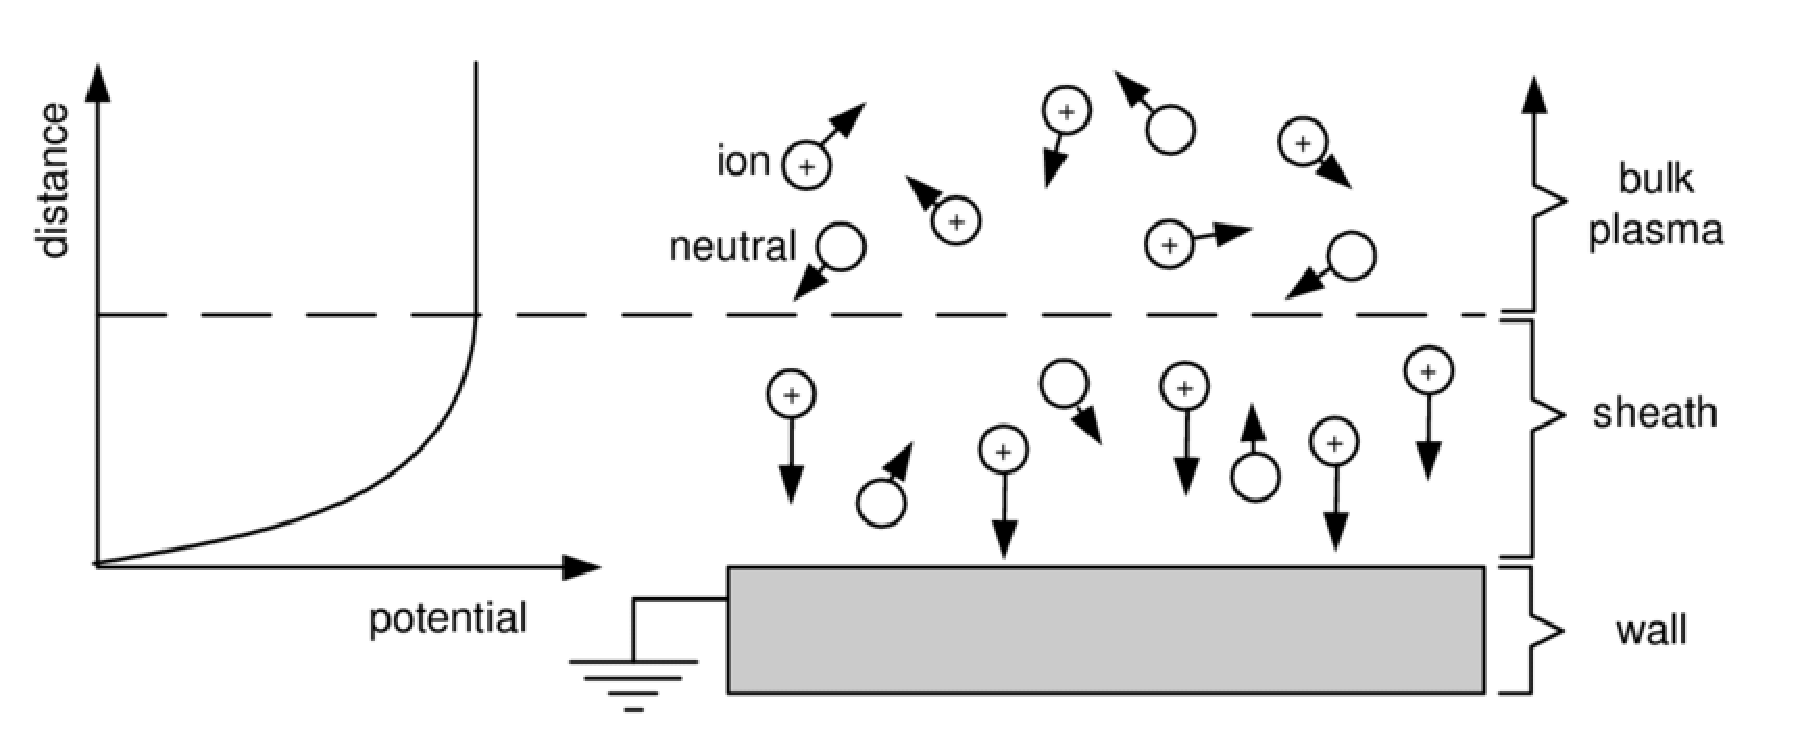
\includegraphics[scale=0.5]{Figures/The-plasma-sheath}
\par\end{centering}
\caption{The plasma sheath. Ions in the plasma happen upon the sheath, where
they are accelerated to the wall. At the wall, ions are neutralized
by electrons from the ground and return to the bulk.}

\end{figure}


\subsection{Collisionless Sheath}

\subsubsection{What is collisionless sheath}

When the ion mean free path is much larger than the sheath thinkness,
the sheath is called a collisionless sheath. Within a collisionless
sheath, the velocites of ions are only determined by the sheath field
and ions are continuously accelerated by the sheath field. Ions pick
up energies as they enter the plasma-sheath edge and exit the sheath
with an energy distribution of a bimodal shape, seen the figure below.
At low frequencies ($\tau_{ion}/\tau_{rf}\ll1$, transverse time of
ion is much smaller than the RF period), the ions traverse the sheath
within a small fraction of an RF cycle. The phase of the RF cycle
at which ions enter the sheath determines their energies at the exit.
In this case, the IED (Ion Energy Distribution) is broad and bimodal,
with the two peaks corresponding to the minimum and maximum of the
sheath drops. At high frequency ($\tau_{ion}/\tau_{rf}\gg1$, transverse
time of ion is much larger than the RF period), it takes the ions
many RF cycles to cross the sheath. In such a scenario, the net energy
gained by the ions is determined by the DC component, which is the
time-averaged sheath voltage. The effect of phase at which they enter
the sheath is significantly reduced. The IED is still bimodal, but
much narrower. 

\begin{figure}[H]
\begin{centering}
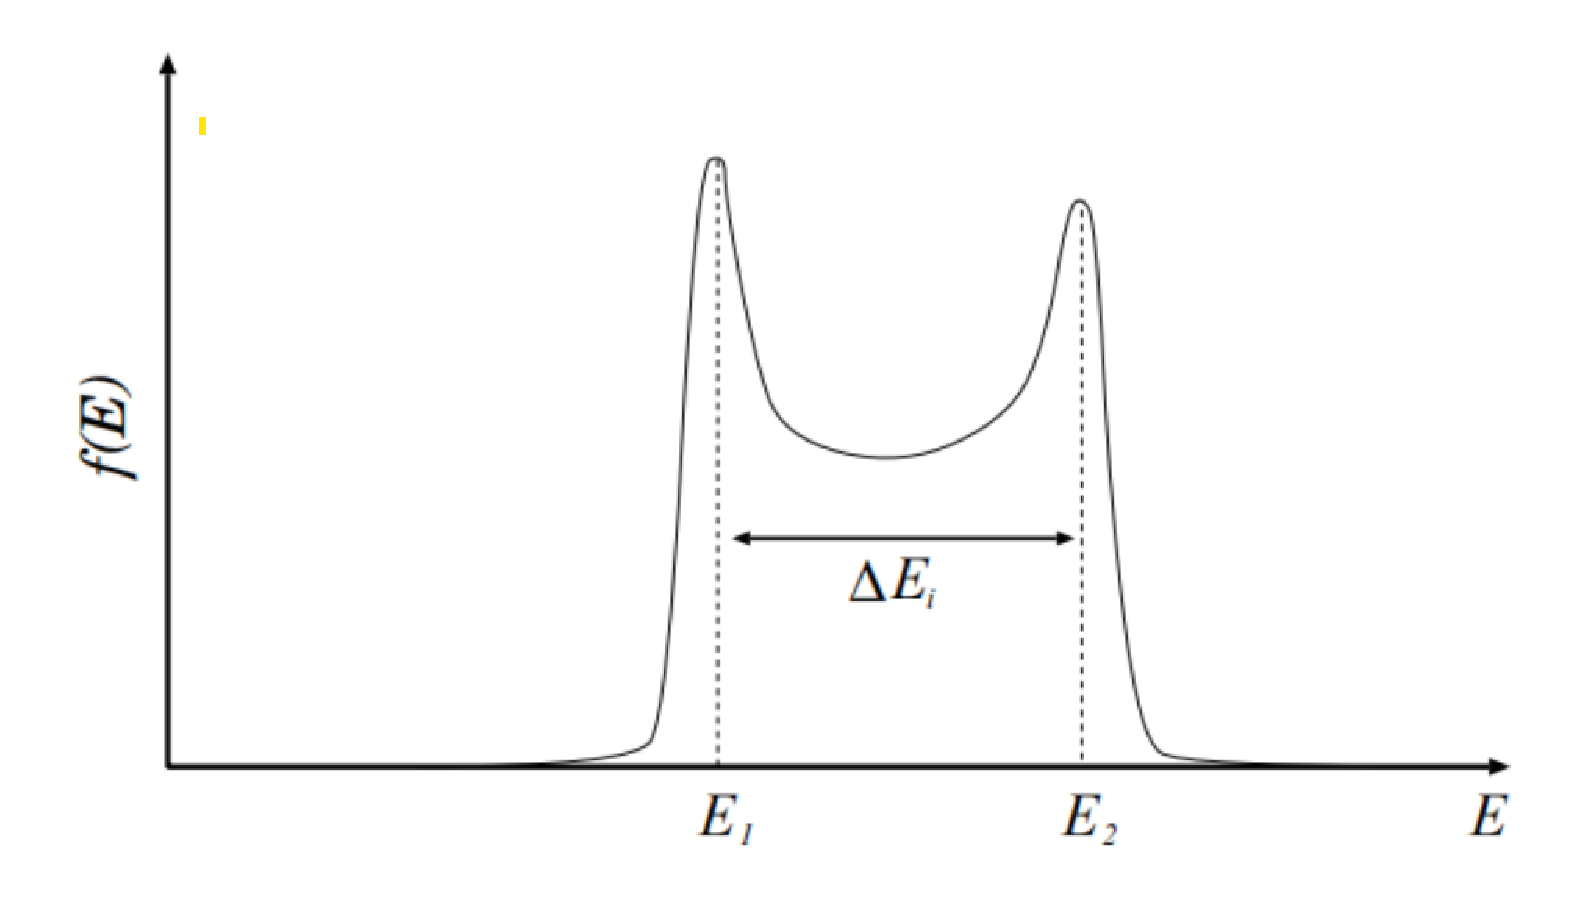
\includegraphics[scale=0.5]{Figures/Bimodal-IED}
\par\end{centering}
\caption{A bimodal ion energy distribution.}

\end{figure}


\subsubsection{Analytic Collisionless Sheath Model}

Benoit-Cattin et al{[}{]} obtained an analytic solution for IED at
the high-frequency regime ($\tau_{ion}/\tau_{rf}\gg1$, transverse
time of ion is much larger than the RF period), assuming 
\begin{enumerate}
\item a constant sheath thickness, $\bar{s}$
\item a uniform sheath electric field, $\vec{E}$is independent of position
$x$ 
\item a sinusoidal sheath voltage $V_{sh}(t)=V_{dc}+V_{s}sin(\omega t)$
\item zero initial ion velocity at the plasma-sheath boundary, $v_{ion}(x=\bar{s})=0$
\end{enumerate}
The resulting expressions for $\Delta E_{i}$and the IED are
\[
\Delta E_{i}=\frac{2eV_{s}}{\bar{s}\omega}(\frac{2eV_{dc}}{m_{i}})^{1/2}=\frac{3eV_{s}}{\pi}(\frac{\tau_{rf}}{\tau_{ion}})
\]
\[
f(E)=\frac{dn}{dE}=\frac{2n_{t}}{\omega\Delta E_{i}}[1-\frac{4}{\Delta E_{i}^{2}}(E-eV_{dc})^{2}]^{-1/2}
\]

where $n_{t}$is the number of ions entering the sheath per unit time.

The calculations yield a bimodal IED with two peaks symmetric about
$eV_{dc}$and $\Delta E_{i}$proportional to $\frac{\tau_{rf}}{\tau_{ion}}$,
seen the figure below.

\begin{figure}[H]
\begin{centering}
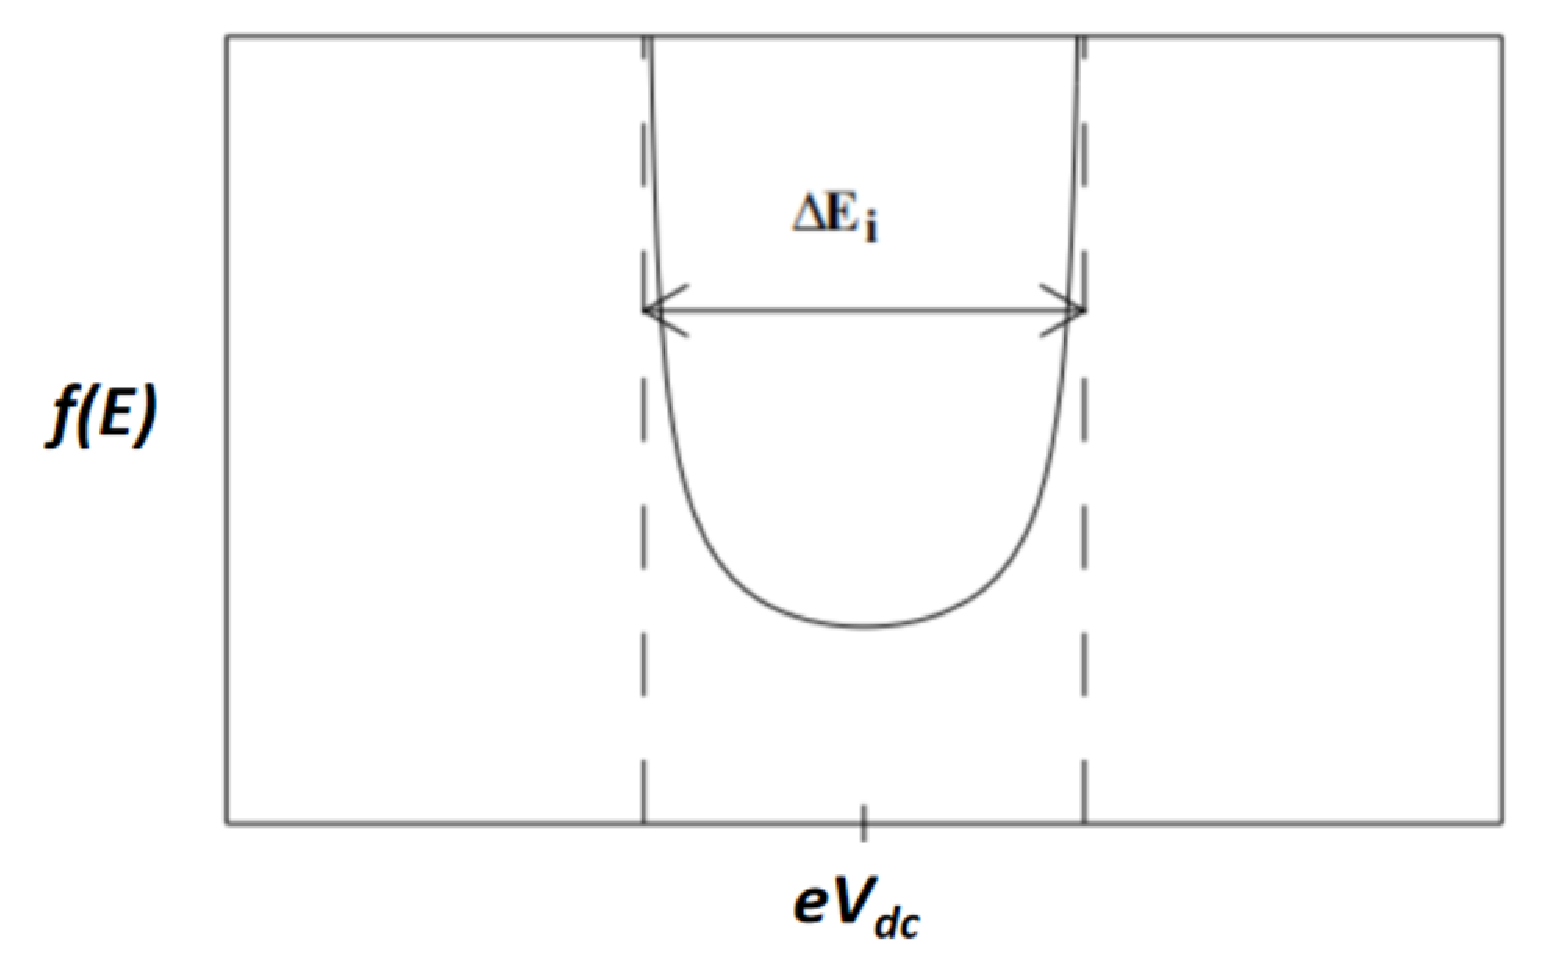
\includegraphics[scale=0.5]{Figures/Bimodal-IED-Analytic}
\par\end{centering}
\caption{The plot of analytic solution for IED at the regime of high frequency
($\tau_{ion}/\tau_{rf}\gg1$) . The singular peaks are due to the
assumption of a mono-energetic initial ion velocity distribution.}

\end{figure}


\subsubsection{Collisionless Sheath Model}

In the collisionless sheath model, we only need to solve the Newton's
euqation, 
\[
\frac{d}{dt}\vec{x}=\vec{v}
\]
\[
\frac{d}{dt}\vec{v}=\frac{eq}{m_{i}}\vec{E}(t)
\]
\[
\vec{E}(\vec{x},t)=f(V_{sh}(x,t),s(t))
\]
\[
\vec{x},\vec{v}-position,velocity
\]
\[
e-elementary\:charge
\]
\[
q-\#\:of\:charges\:carried\:by\:ion
\]
\[
\vec{E}(\vec{x},t)-electric\:field\:within\:sheath
\]
\[
V_{sh}(\vec{x},t)-sheath\:potential
\]
\[
s(t)-sheath\:thickness
\]


\subsection{Collisional Sheath}

When the mean free path of ions, $\lambda_{ion}$, is much smaller
than the sheath thickness, the ions entering the sheath will experience
collisions before exit. Collisions can alter the velocity, both speed
and angle. The probability of a collision event occurring depends
on the ion-neutral collision frequency, $v_{in}$, which is defined
as:
\[
v_{in}=N_{d}\sigma|\vec{v}_{i}-\vec{v}_{g}|
\]
\[
N_{d}-backgroud\:number\:density
\]
\[
\sigma-ion-neutral\:charge\:exchange\:collision\:cross\:section
\]
\[
\vec{v}_{i},\vec{v}_{g}-ion\:velocity,\:background\:gas\:velocity
\]

The collision probability defined as 
\[
P=1-exp(-v_{in}\Delta t)=1-exp(-\frac{\Delta x}{\lambda_{ion}})
\]


\subsection{Analytic Sheath Model}

\section{Feature Model}

\subsection{Introduction}

\begin{onehalfspace}
The Langmuir Feature Model uses particle-based Monte Carlo methods
to simulate the evolution of etch features when exposed to plasma
discharges. The model uses pseudo-particles to represent the incoming
species, including electron, ions and neutral particles. All these
pseudo-particles are tracked for their trajectories and interactions
with materials. The materials in the model are represented by a structured
mesh of voxels or cubes. Each voxel or cube represents a macro solid
material, which consists of hundreds of atoms or molecules. The mesh
can be initialized in an arbitrary shape with surface conditions,
which may include multiple materials and features within the each
domain. This allows the simulation of complex structures and steps
in the fabrication process, such as finFET structure. 

A pseudo-particle is also a macro particle, which consists of atoms
or molecules with the same number as in the materials. The pseudo-particles
are launched with specified flux, angle and energy, which are often
derived from a reactor scale model, which is, within the Langmuir
Model, the Langmuir Reactor Model. Without the reactor model, the
Langmuir Feature Model can also self generate generic functions of
flux, angle and energy. The coupling of feature scale model to reactor
scale model allows the Langmuir Model to explore the process recipe
with the etch result, or to be used to study fundamental physics.
This versatility makes the Langmuir Model a strong tool for recipe
tuning and optimization, as well as new physics investigation.
\end{onehalfspace}

\subsection{Mesh - 2D}

\begin{onehalfspace}
The mesh in Langmuir Feature Model is constructed in 2D space, in
which $(x,z)$ are used to represent the 2D coordinates and infinity
is assumed in $y$ direction. The model discretizes the 2D space into
a rectangular computational cells. The cell center is marked as a
node, which determines the location $(x,z)$ of the cell. Each cell
has a volume of $\Delta x\times\Delta z$, where $\Delta x$ and $\Delta z$
are the resolutions in $x$ and $z$ directions, respectively. Usually,
square cells, where $\Delta x=\Delta z$, are used. Non-square cells,
which are used for high aspect ratio domain for memory saving, need
future test and validation. The computational complexity increases
with reducing resolution as approximately $O(n^{3})$, where $n$
is the number of cells per side in the simulation domain. The choice
of resolution also affects the time weighting of each pseudo-particle,
which will be described later.

Each cell, representing a solid material, is assigned a material property.
The most commonly used materials, Such as $Si$ and $SiO_{2}$, in
the Langmuir Feature Model are pre-defined in the database coming
along with the model. If not found in the database, the materials
can be defined by the user. The materials are used for the chemical
reactions. It is important to respect stoichiometry, and most materials
are defined as elements or compounds to facilitate this, but there
is no inherent limitation on the material properties in the model.
It means that arbitrary materials can be built upon simulation request.
In that case, the user is responsible for the validity of the physics
and chemistry represented by the model. An example of an arbitrary
material definition is ``\textit{Photo Resist}'', which is commonly
used as a etching mask. ``\textit{Photo Resist}'' is a polymer with
multiple elements and complicated structures, where a long chain of
molecules could surpass the cell size. It is okay for these resists
to have varying chemistries and properties, and it is not always possible
or necessary to capture their stoichiometry accurately.

The basic element in the mesh is a cell, which is assigned a single
material and not dividable. Each solid cell in the mesh is assumed
to have the same atomic denisty, $\rho\;cm^{-3}$, which is typically
$5.0\times10^{22}\;cm^{-3}$ for $Si$ and $2.3\times10^{22}\;cm^{-3}$
for $SiO_{2}$. This density is a user input and used to calculate
number of atoms per cell, 
\[
N_{cell}=\Delta x\times\Delta z\times\rho
\]
 Because all cells contain a single (usually stoichiometric) material,
but are represented as having the same volume and denisty, it is important
to keep in mind that all materails in the Langmuir Feature Model represent
average behaviors of their respective coupounds. The Langmuir Feature
Model is designed to address the nano-scale feature during the fabrication
process, but not able to resolve the inter-atomic interactions. To
apply the model within the valid window, the user should make sure
that $N_{cell}\gg1$, which will not be automatically checked in the
model. 
\end{onehalfspace}

\subsection{Pseudo-Particle}

\subsubsection{Definition of the pseudo-particle}

Simulating a single ion or radical coming to the feature is not practical
due to the huge computational cost. During a typical etching process,
the ion flux coming to the wafer is of $10^{16}\;cm^{-2}s^{-1}$,
while radical flux of $10^{18}\;cm^{-2}s^{-1}$. In a feature domain
of $100nm\times100nm$ for a process of $10s$, there are$10^{7}$
ions and $10^{9}$ radicas needed to be launched and tracked, which
is clearly beyond the capability of any existing computer or cluster.
Instead of a single particle, a macro-particle called pseudo-particle
and designed like the material cell, is used in the Langmuir Feature
Model. A pseudo-particle consists of $N_{cell}$ identical particles,
which could be electorn, ions, neutals or even photons. Each pseudo-particle
is assigned the properties of a single species and not dividable.
The number density of a pseudo-particle matches the material cell
so that any reactions occur between them are balanced and act as single-particle
reactions.

\subsubsection{Particle Launch}

In a time period $T$, the total launched pseudo-particles, $N_{particle}\times N_{cell}$,
needs to match the total fluence, $Flux\times Aera\times T$, into
the domain. In average, each pseudo-particle occupies a time duration
of 
\[
\Delta t=\dfrac{N_{cell}}{Flux\times Area}
\]
By considering the average velocity of the pseudo-particle and the
domain of the feature, the life time of a pseudo-particle is about
\[
t_{life}=\dfrac{L\times N_{reflect}}{V_{particle}}
\]
where $L$ is the characterstic length of the domain, $L<\sqrt{width^{2}+height^{2}}$,
$N_{reflect}$ is the number of reflections experienced by the pseudo-particle,
$N_{reflect}<10$ for most scenarios, $V_{particle}$ is the average
speed of the pseudo-particle, $t_{life}$ is the lifetime of a pseudo-particle.
Let us put those numbers into an example case. $L=100\:nm$ for a
domain of $100\:nm\times100\:nm$, $N_{reflect}=10$, and $V_{particle}=500\:m/s=500\:nm/ns$
at room temperature. The resulting $t_{life}=2\:ns$ is far smaller
than typical $\Delta t=100\:ns$. It means that a pseudo-particle
is lauched and gets dead before next pseudo-particle is launched,
which indicates that no interaction of pseudo-particles is necessary
to be taken into account. The only interacting object of a pseudo-particle
is the material cell. The summary of the important assumptions can
be seen as below:
\begin{itemize}
\item Pseudo-particles uniformly enter the feature. This indicates that
each pseudo-particle occupies exact $\Delta t$, defined as above.
\item A pseudo-particle entering the feature is a rare event. This implies
that each pseudo-particle event is instantaneous compared to the time
between incoming pseudo-particle. Pseudo-particles do not interact
with each other.
\item The number of total pseudo-particle entering the feature per area
and per time is exactly the same as the flux. This ensures that the
overall effects of total pseudo-particles well align with the physics
requirements.
\end{itemize}
The first assumption can be argued as the real entering events could
follow Poisson's distribution more than uniform distribution. Even
under the assumption of Poisson's distribution, you could find the
event of two pseudo-particles entering the feature with overlap in
time is rare. Compared to millions of pseudo-particles launched in
a simulation, the first two assumptions together still hold. 

\subsubsection{Particle Tracking without E-field}

In the serial version of Langmuir Feature Model, all pseudo-particles
are launched in sequence and particle tracking is only applied to
a single particle each time. In the terms of memory management, a
memory space is created initially for a single pseudo-particle. When
a pseudo-particle dies, a new pseudo-particle can reuse the memory
space by updating the particle properties, such as position and velocity.
The pseudo-particles are by default launched from the top boundary
fo the domain. The initial position of pseudo-particle is randomly
picked. The velocity vector, consisting of speed and angle w.r.t.
$x=0^{+}$, is chosen randomly from the given distribution. The given
distribution could be either generated from the feature model itself,
or from the IAEDF generated from the Langmuir Reactor Model. 

Without E-field, a pseudo-particle is not accelerated during the flight.
It means that the pseudo-particle follows the line--of-sight trajectory.
Although the geometry is meshed to grids, the pseudo-particle advances
in continous space. Newton's equations are solved for the trajectory,
\[
\vec{r}=\vec{r}+\vec{v}\times dt
\]

where $\vec{v}$ and $\vec{r}$ are the velocity and position of the
pseudo-particle, respectively. $dt$ is the flight timestep, which
is far smaller than the simulation timestep. Instead of integrating
over flight timestep $dt$, a advancing step, $\Delta L$ , is used
in Langmuir Feature Model,
\[
\vec{r}=\vec{r}+\vec{v}_{unit}\times\Delta L
\]

where $\vec{v}_{unit}$ is the normalized unit vector of the velocity
and $\Delta L$ is the advance step. Typical $\Delta L$ is constant
and set to be about the resolution of the mesh. Larger $\Delta L$
definitely reduces the computing time. A varying $\Delta L$, which
is determined by the position, can be used and will be discussed separately.
 

\subsubsection{Particle Tracking with E-field}

When E-field is taken into account, velocity for charged particles
is not constant anymore. Full Newton's equations need to be solved,
\[
\vec{v}(t+dt)=\vec{v}(t)+\dfrac{q\vec{E}}{m}dt
\]
\[
\vec{r}=\vec{r}+\vec{v}\times dt
\]

where $\vec{E}$ is the E-field, $q$ is the particle charge, and
$m$ is the particle mass. In the feature model, E-field is a function
of position and changes with deposited surface charges. Within the
tracking of a single particle, E-field does not change with time.
Therefore, Newton's equations can be solved using spacestep instead
of timestep,
\[
\vec{v}(\vec{r}+d\vec{r})=\vec{v}(\vec{r})+\dfrac{q\vec{E}}{m}\times\dfrac{\Delta L}{abs(\vec{v})}
\]
\[
\vec{r}=\vec{r}+d\vec{r}
\]
\[
d\vec{r}=\vec{v}_{unit}\times\Delta L
\]

The chosen of $\Delta L$ depends on the spatial variation of E-field.
In general, if the gradient of E-field is small, $\Delta L$ can be
increased; vice versa. In most cases, $\Delta L$ should not be larger
than the resolution of the mesh.

\subsubsection{Ray Tracing}

To be added.

\subsection{Particle-Materials Interactions}

\subsubsection{Hit Check}

When the particle is tracked by step advance algorithm, particle-materail
collision needs to be checked. In Langmuir Feature Model, there is
no volume assinged to the pseudo-particle, which means that particle
trajectory is an 1D line. At a fixed time, the pseudo-particle is
a point without any dimemsions. When the pseudo-particle gets inside
a material cell, the model flags a ``Hit''. ``Inside a cell''
means that the position $(x,z)$ of the particle lies within the boundary
of the cell,
\[
C_{left}<x<C_{right}
\]
 
\[
C_{bottom}<z<C_{top}
\]
where $C_{left}$, $C_{right}$, $C_{bottom}$ and $C_{top}$ are
the four boundaries for a cell. In the program, in stead of checking
the four boundaries, the particle is mapped onto the computational
mesh of materials using, 
\[
i=int(x-0.5\Delta x)
\]
\[
j=int(z-0.5\Delta z)
\]

It means that the particle is now within the cell $C(i,j)$. If $C(i,j)$
is vacuum, then the particles continues to advance. Otherwise, the
particle is considered to hit the material cell, $C(i,j)$. 
\end{document}
